\newpage
\section{Analisi statistica FastJson}

\subsection{Analisi Statistica Technical Debt}
In \autoref{td_AnalisiFastJson-tipo} è possibile osservare la dimensione del technical debt rispetto alla tipologia di clone. L'analisi statistica è confermata dal p-value, ottenuto con il test di Kruskal-Wallis mediante R, che ha un valore inferiore a $2,2 e^{-16}$.
\begin{figure}[htbp]
	\centering
	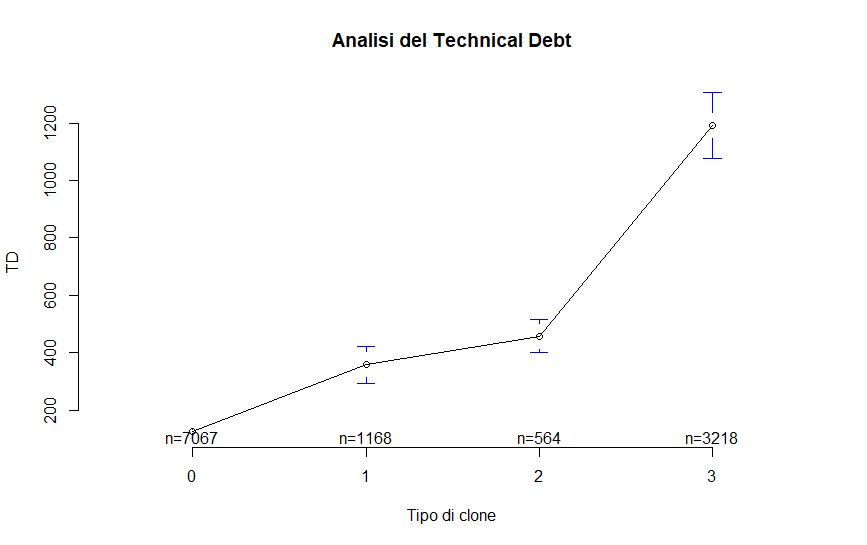
\includegraphics[scale=0.5]{analisi_R/AnalisiFastJson/1-gplot-td-type.png}
\caption{Analisi statistica Technical Debt FastJson}
\label{td_AnalisiFastJson-tipo}
\end{figure}
Il grafico in figura \autoref{td_AnalisiFastJson-tipo} presenta sull'asse delle ascisse il tipo di clone, indicando con zero le classi in cui il codice clonato è assente. Si riporta, invece, sull'asse delle ordinate il valore del technical debt. Si indica con n il numero delle occorrenze dei cloni di ciascun tipo presenti nelle quattro versioni del progetto. Essendo un'analisi statistica, si rapporta il technical debt totale al numero di occorrenze complessive dei cloni. In questo caso l'analisi statistica conferma l'ipotesi fatta, cioè che i cloni di tipo 3 hanno un technical debt maggiore rispetto alle altre tipologie di cloni, poiché le occorrenze complessive dei tipi di cloni hanno ordini di grandezza non molto distanti tra loro.

\subsection{Analisi Statistica Code Smells}
In \autoref{codesmell_AnalisiFastJson-tipo} è possibile osservare la quantità di code smells rispetto alla tipologia di clone. L'analisi statistica è confermata dal p-value, ottenuto con il test di Kruskal-Wallis mediante R, che ha un valore inferiore a $2,2 e^{-16}$. \newpage
\begin{figure}[htbp]
	\centering
	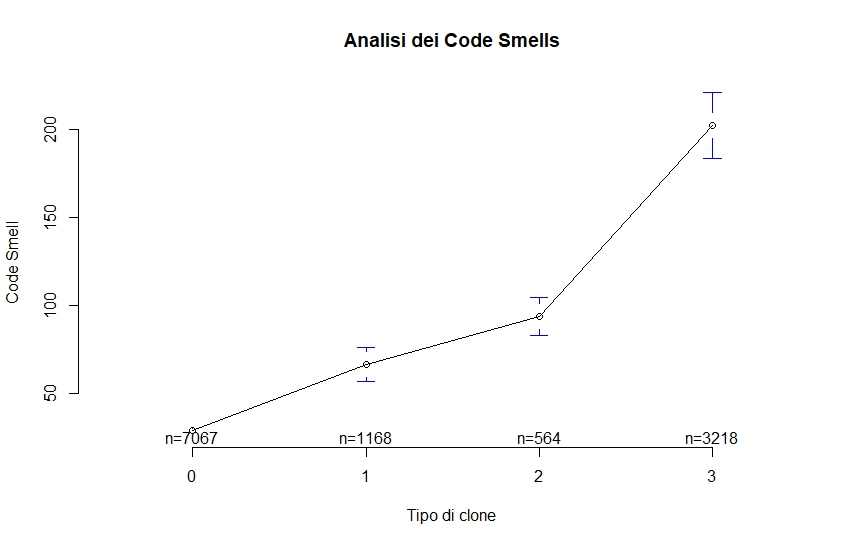
\includegraphics[scale=0.5]{analisi_R/AnalisiFastJson/2-gplot-codesmell-type.png}
\caption{Analisi statistica Code Smell}
\label{codesmell_AnalisiFastJson-tipo}
\end{figure}
Il grafico in figura \autoref{codesmell_AnalisiFastJson-tipo} presenta sull'asse delle ascisse il tipo di clone, indicando con zero le classi in cui il codice clonato è assente. Si riporta, invece, sull'asse delle ordinate il valore dei code smells. Si indica con n il numero delle occorrenze dei cloni di ciascun tipo presenti nelle quattro versioni del progetto. Essendo un'analisi statistica, si rapporta in numero di code smells totali al numero di occorrenze complessive dei cloni. In questo caso l'analisi statistica conferma l'ipotesi fatta, cioè che i cloni di tipo 3 hanno un numero di code smells maggiore rispetto alle altre tipologie di cloni, poiché le occorrenze complessive dei tipi di cloni hanno ordini di grandezza non molto distanti tra loro.

\subsection{Analisi Statistica Lunghezza Codice Clonato}
In \autoref{len_AnalisiFastJson-tipo} è possibile osservare la lunghezza del codice clonato (espressa in LOC) rispetto alla tipologia di clone. L'analisi statistica è confermata dal p-value, ottenuto con il test di Kruskal-Wallis mediante R, che ha un valore inferiore a $6,295e^{-11}$. \newpage
\begin{figure}[htbp]
	\centering
	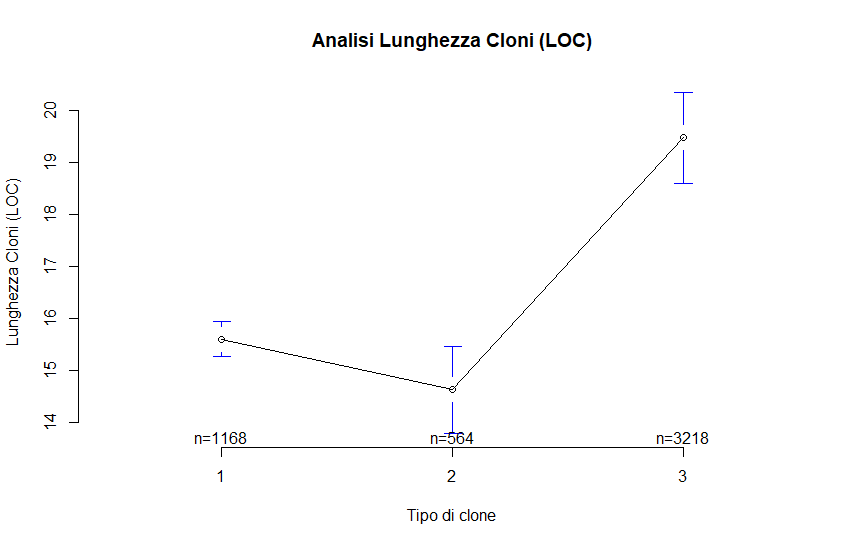
\includegraphics[scale=0.5]{analisi_R/AnalisiFastJson/3-gplot-len-type.png}
\caption{Analisi statistica Lunghezza Codice Clonato }
\label{len_AnalisiFastJson-tipo}
\end{figure}
Il grafico in figura \autoref{len_AnalisiFastJson-tipo} presenta sull'asse delle ascisse il tipo di clone. Si riporta, invece, sull'asse delle ordinate la lunghezza dei cloni espressa in LOC. Si indica con n il numero delle occorrenze dei cloni di ciascun tipo presenti nelle quattro versioni del progetto. Essendo un'analisi statistica, si rapporta in numero di code smells totali al numero di occorrenze complessive dei cloni. Si nota che i cloni di tipo 3 hanno una lunghezza maggiore rispetto ai cloni di tipo 1 e 2.